\renewcommand{\theequation}{\theenumi}
\begin{enumerate}[label=\thesubsection.\arabic*.,ref=\thesubsection.\theenumi]
\numberwithin{equation}{enumi}
	%
\item Any point $\vec{P}$ in the 2-D plane can be expressed in terms of its coordinates $\brak{p_1,p_2}$ as the column vector
\begin{align}
\vec{P} = \myvec{p_1\\p_2}
\end{align}
%%
\item The {\em direction vector} of the line joining $\vec{P}, \vec{Q}$ is defined as 
\begin{align}
\label{eq:dir_vec}
\vec{m} &= \vec{P}-\vec{Q} = \myvec{p_1-q_1\\p_2-q_2}
\\
&= \brak{p_1-q_1}\myvec{1 \\\frac{p_2-q_2}{p_1-q_1}} = 
\brak{p_1-q_1}\myvec{1 \\m}  
\end{align}
%
where 
\begin{align}
m = \frac{p_2-q_2}{p_1-q_1}.
\end{align}
{\em Without loss of generality, $k\vec{m}$, for any real scalar $k$ is also a direction vector.  In the rest of the paper, $\vec{m}$ and $k\vec{m}$ are interchanged for computational simplicity}.  Thus, if $m$ be the slope of the line $PQ$,
\begin{align}
\label{eq:dir_vec_slope}
\vec{m} = \myvec{1 \\ m}
\end{align}
%
\item Let $\vec{P},\vec{Q}$ be two points on a line.  The vector equation of the line is given by
\begin{align}
\label{eq:line_param}
\vec{x} &= \vec{P} + \lambda \vec{m}, \quad \lambda \in \mathbb{R}
\\
\vec{m} &= \vec{P}-\vec{Q}
\end{align}
\eqref{eq:line_param} can be used in 3D as well.
%
\item The {\em normal vector} $\vec{n}$ to a line is orthogonal to the direction vector $\vec{m}$ so that
\begin{align}
\label{eq:line_dir_norm}
\vec{m}^T\vec{n} = 0
\end{align}
%
If $\vec{P}$ be a point on the line, the equation of the line can be expressed as
\begin{align}
\label{eq:line_norm_eq}
\vec{n}^T\brak{\vec{x}-\vec{P}} &= 0
\\
\text{or, } \vec{n}^T\vec{x} &= c,
\label{eq:line_norm_eq_c}
\end{align}
%
where
\begin{align}
c = \vec{n}^T\vec{P}
\end{align}
which is the desired  equation of the straight line.  By subsuming the $c$ in \eqref{eq:line_norm_eq_c} within $\vec{n}$, the equation of a line can also be expressed as
\begin{align}
\label{eq:line_norm_eq_unit}
\vec{n}^T\vec{x} &= 1
\end{align}
%
Note that in 3D, \eqref{eq:line_norm_eq} and \eqref{eq:line_norm_eq_c} are used to represent the equation of a plane. 

\item {\em Orthogonality: }Show that the points
\begin{align}
\vec{A} = \myvec{2\\-1\\1}, 
\vec{B} = \myvec{1\\-3\\-5}, 
\vec{C} = \myvec{3\\-4\\-4} 
\end{align}
%
are the vertices of a right angled triangle.
\\
\solution Let 
\begin{align}
\vec{v}_1 &= \vec{A}-\vec{C} = \myvec{-1\\3\\5} 
\\
\vec{v}_2 &= \vec{B}-\vec{C} = \myvec{-2\\1\\-1} 
\end{align}
Then 
\begin{align}
\vec{v}_1^T\vec{v}_2  &=  \myvec{-1&3&5}  \myvec{-2\\1\\-1} =0
\\
\implies AC &\perp BC
\end{align}
and $\vec{v}_1$ and $\vec{v}_2$ are said to be orthogonal. 

\item  Find the equation of the line through \myvec{- 2\\ 3} with slope - 4 
%\cite{eleven}.
\label{prob:lineq}
%
\begin{figure}
\centering
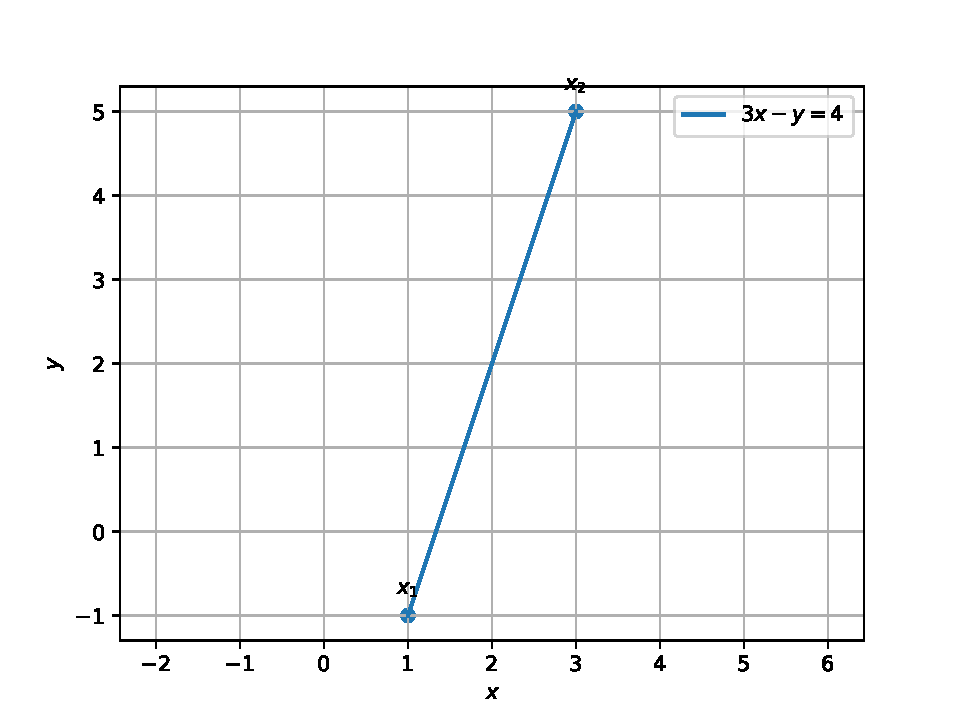
\includegraphics[width=\columnwidth]{./figs/line/line_points.eps}
%}%
\caption{ Line obtained in Problem \ref{prob:lineq}.}%
\label{fig:line_equation}
\end{figure}
\\
\solution From \eqref{eq:dir_vec_slope}, the direction vector is
\begin{align}
\label{eq:lineq_dir}
\vec{m} = \myvec{1\\-4}
\end{align}
and from \eqref{eq:line_dir_norm}, the normal vector is
\begin{align}
\label{eq:lineq_norm}
\vec{n} = \myvec{4\\1}
\end{align}
Using \eqref{eq:line_norm_eq}, the equation of the line is 
\begin{align}
\label{eq:lineq_norm_arith}
\myvec{4 &1}\cbrak{\vec{x}-\myvec{- 2\\ 3}} &= 0
\\
\implies \myvec{4 &1}\vec{x} &= -5
\label{eq:lineq_norm_final}
\end{align}
Fig. \ref{fig:line_equation} shows the line passing through the given point.

\item  Write the equation of the line through the points $\vec{x}_1=\myvec{1\\-1}$ and $\vec{x}_2 = \myvec{3\\5}$. 
\label{prob:line_plane}
\begin{figure}
\centering
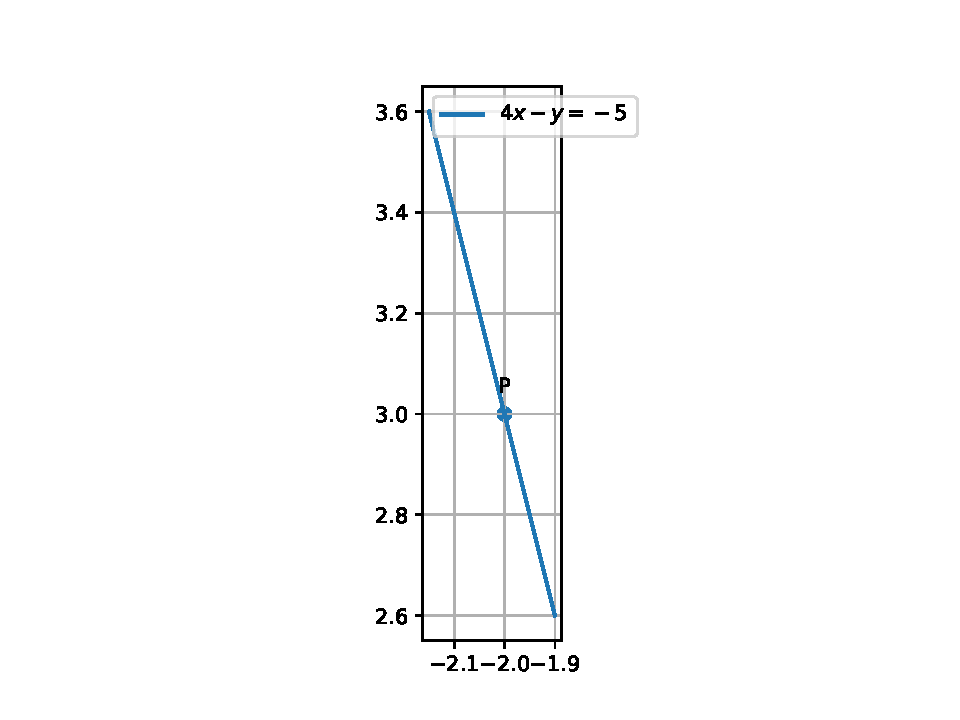
\includegraphics[width=\columnwidth]{./figs/line/line_slope.eps}
\caption{ Line obtained in Problem 
\ref{prob:line_plane}.}
\label{fig:line_plane}
\end{figure}
\\
\solution 
 From \eqref{eq:line_norm_eq_unit},  
\begin{align}
\vec{n}^T\myvec{1 \\ -1} &= 1
\\
\vec{n}^T\myvec{ 3 \\ 5}  &= 1
\end{align}
%
resulting in the the matrix equation
\begin{align}
\myvec{1 & -1 \\ 3 & 5} \vec{n} = \myvec{1 \\ 1}
\end{align}
yielding the augmented matrix
\begin{align}
\myvec{1 & -1 & 1 \\ 3 & 5 & 1} 
\end{align}
Performing row reduction,
\begin{align}
\myvec{1 & -1 & 1 \\ 3 & 5 & 1} 
\\
\xleftrightarrow {R_2\leftarrow R_2 -3R_1}\myvec{1 & -1 & 1\\0 & 8 & -2} 
\\
\xleftrightarrow {R_2\leftarrow \frac{R_2}{2}}\myvec{1 & -1 & 1\\0 & 4 & -1} 
\\
\xleftrightarrow {R_1\leftarrow 4R_1+R_2}\myvec{4 & 0 & 3\\0 & 4 & -1} 
\\
\xleftrightarrow [R_1\leftarrow\frac{R_1}{4}]{R_2\leftarrow \frac{R_2}{4}}\myvec{1 & 0 & \frac{3}{4}\\0 & 1 & -\frac{1}{4}} 
\label{eq:line_aug}
\end{align}
From \eqref{eq:line_aug},
\begin{align}
\vec{n} = \frac{1}{4}\myvec{3 \\-1}
\end{align}
%
Thus the equation of the desired line is 
\begin{align}
\frac{1}{4}\myvec{3 &-1}\vec{x} &= 1
\\
\text{or, } \myvec{3 &-1}\vec{x} &= 4
\end{align}
Fig. \ref{fig:line_plane} shows the line passing through the given points.
\item  ({\em Linear Dependence}) Prove that the three points $\myvec{3\\0},\myvec{-2\\-2},\myvec{8\\2}$ are collinear 
\label{prob:points_collinear}
\begin{figure}
\centering
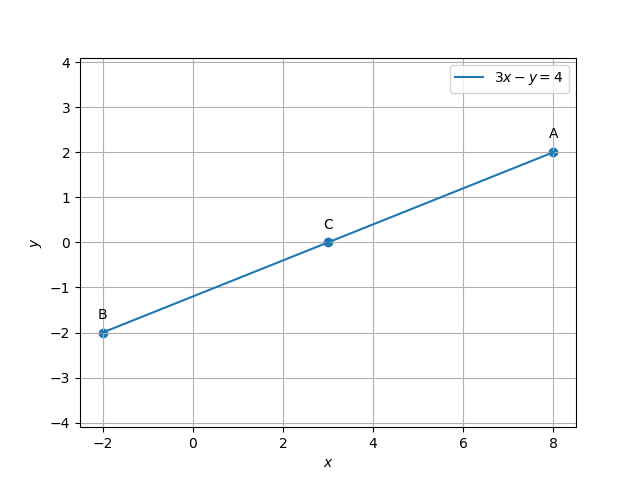
\includegraphics[width=0.4\columnwidth]{./figs/line/points_collinear.eps}
\caption{ Points on a line and points forming a triangle in Example \ref{prob:points_collinear}.}%
\label{fig:line_collinear}
\end{figure}
%\cite{eleven}.
\\
\solution 
Let
\begin{align}
\begin{split}
\vec{v}_1 &= \myvec{3\\0}-\myvec{-2\\-2} = \myvec{5\\2}
\\
\vec{v}_2 &=\myvec{-2\\-2}-\myvec{8\\2} = \myvec{-10\\-4}
\end{split}
\label{eq:lin_dep_vecs}
\end{align}
Then, the given points are collinear if 
\begin{align}
\label{eq:lin_dep}
x_1\vec{v}_1+x_2\vec{v}_2 &= 0 
\end{align}
has a nontrivial solution as well, i.e.
\begin{align}
\vec{x} =\myvec{x_1\\x_2} \ne \vec{0}
\end{align}
Substituting \eqref{eq:lin_dep_vecs}
in \eqref{eq:lin_dep} results in the matrix  equation
\begin{align}
\myvec{5 & -10\\ 2 & -4}\vec{x} = 0
\end{align}
Performing row operations on the matrix,
\begin{align}
\myvec{5 & -10\\ 2 & -4}
\xleftrightarrow[]{R_2\leftarrow 2R_1-5R_2}
\myvec{5 & -10\\ 0 & 0}
\end{align}
which can be expressed as
%
\begin{align}
\myvec{5 & -10}\vec{x} &= 0
\\
\text{or, } \vec{x} &= x_1\myvec{1\\-2}
\end{align}
Thus, there are infinite solutions.  The vectors $\vec{v}_1, \vec{v}_2$ are are linearly dependent and the given points  lie on a straight line.
\item Alternatively, if the given points are collinear, from \eqref{eq:line_norm_eq_unit},
\begin{align}
\label{eq:collinear_2d}
\myvec{3&0 \\ -2&-2 \\ 8&2} \vec{n} &= \myvec{1\\1\\1}
\end{align}
Row reducing the augmented matrix,
\begin{align}
\myvec{3&0 & 1\\ -2&-2 & 1\\ 8&2 & 1} 
\\
\xleftrightarrow[R_2\leftarrow 3R_2+2R_1]{R_3\leftarrow 3R_3-8R_1}
\myvec{3&0 & 1\\ 0&-6 & 5\\ 0&6 & -5}
\\
 \xleftrightarrow[]{R_3\leftarrow R_3+R_2}\myvec{3&0 & 1\\ 0&6 & -5\\ 0&0 & 0}
\end{align}
The above matrix has a zero row in echelon form, hence \eqref{eq:collinear_2d}
is consistent and the given points are on a straight line. Also,
\begin{align}
\vec{n} = \frac{1}{6}\myvec{2\\-5}
\end{align}
\item ({\em Linear Independence}) Do the points $\myvec{3\\2},\myvec{-2\\-3},\myvec{2\\3}$ form a triangle?
\label{prob:points_triangle}
\begin{figure}
\centering
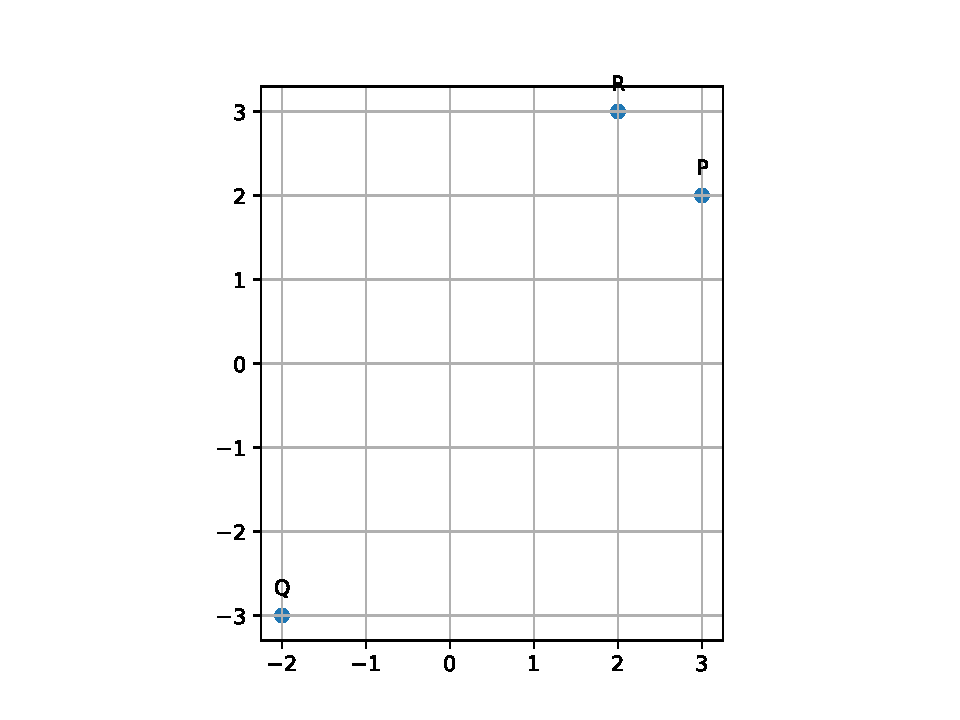
\includegraphics[width=\columnwidth]{./figs/line/points_triangle.eps}
\caption{ Points on a triangle in Problem \ref{prob:points_triangle}.}%
\label{fig:points_triangle}
\end{figure}
\\
\solution In this case
\begin{align}
\vec{v}_1 &= \myvec{3\\2}-\myvec{-2\\-3}=\myvec{5\\5}
\\
\vec{v}_2 &= \myvec{-2\\-3}-\myvec{2\\3} = \myvec{-4\\-6}
\end{align}
Thus,
\begin{align}
\label{eq:lin_indep}
x_1\vec{v}_1+x_2\vec{v}_2 &= 0 
\\
\implies \myvec{5 & -4 \\ 5 & -6}\vec{x} & = 0
\end{align}
Using row operations,
\begin{align}
\myvec{5 & -4\\ 5 & -6}
\xleftrightarrow[]{R_2\leftarrow R_1-R_2}
\myvec{5 & -4\\ 0 & 2}
\\
\xleftrightarrow[]{R_1\leftarrow R_1+2R_2}
\myvec{5 & 0\\ 0 & 2}
\end{align}
resulting in a {\em full rank} matrix.  Hence, 
\begin{align}
 \vec{x} = 0
 \end{align}
and $\vec{v}_1$ and $\vec{v}_2$ are {\em linearly independent}.  The points lie on a triangle.
\item Alternatively, from \eqref{eq:line_norm_eq_unit}, row reducing the augmented matrix
\begin{align}
\myvec{3&2 & 1\\ -2&-3 & 1\\ 2&3 & 1} \xleftrightarrow[]{R_3\leftarrow R_3+R_2}
\myvec{3&2 & 1\\ -2&-3 & 1\\ 0&0 & 2}
\end{align}
The above matrix has a nonzero row in echelon form, hence the given points
do not lie on a straight line.  So they lie on a triangle.
\item  Find the angle between the lines 
%\cite{eleven}
%
\begin{align}
\begin{split}
\myvec{1 & – \sqrt{3}}\vec{x}  &= 5
\\
\myvec{\sqrt{3} & –1}\vec{x}  &= -6. 
\end{split}
\label{eq:inner_prod_prob}
\end{align}
\\
\solution
The angle between the lines can be expressed in terms of the normal vectors 
\begin{align}
\vec{n}_1 = \myvec{1 \\ – \sqrt{3}},  
\vec{n}_2 =\myvec{\sqrt{3} \\ –1}
\end{align}
as
%
\begin{align}
\label{eq:vec_angle}
\cos \theta &= \frac{\vec{n}_1^T\vec{n}_2}{\norm{\vec{n}_1}\norm{\vec{n}_2}}
\\
&= \frac{\sqrt{3}}{2} \implies \theta = 30\degree
\end{align}
\item Find the projection of the vector 
\begin{align}
\label{eq:proj_a}
\vec{a} = \myvec{2\\3\\2}
\end{align}
on the vector
\begin{align}
\label{eq:proj_b}
\vec{b}=\myvec{1\\2\\1}.
\end{align}
\solution 
%
If the angle between the vectors be $\theta$, the projection is defined as 
\begin{align}
\proj{b}{a} = 
\brak{\norm{\vec{a}}\cos\theta} \frac{\vec{b}}{\norm{\vec{b}}}
=  \frac{\brak{\vec{a}^T\vec{b}}}{\norm{\vec{b}}^2}\vec{b}
\end{align}
Substituting the values from \eqref{eq:proj_a}
 and \eqref{eq:proj_b},
\begin{align}
\proj{b}{a} = \frac{5}{3}\myvec{1\\2\\1}
\end{align}
\item ({\em Reflection }) Assuming that straight lines work as a plane mirror for a point, find the image of the point $\vec{P}=\myvec{1\\2}$ in the line 
%
\begin{align}
L: \quad \myvec{1 & -3}\vec{x}  = -4.
\end{align}
\solution From the given equation, the line parameters are
\begin{align}
\vec{n} = \myvec{1 \\ -3}, c =  -4, \vec{m} = \myvec{3 \\ -1}
\end{align}

Let $\vec{R}$ be the reflection of $\vec{P}$ such that $PR$ bisects the line $L$ at $\vec{Q}$. Then $\vec{Q}$ bisects $PR$.  
This leads to the following equations
\begin{align}
\label{eq:reflect_bisect}
2\vec{Q} &= \vec{P}+\vec{R}
\\
\label{eq:reflect_Q}
\vec{n}^{T}\vec{Q} &= c \quad \because \vec{Q} \text{ lies on the given line}
\\
\label{eq:reflect_R}
\vec{m}^{T}\vec{R} &= \vec{m}^{T}\vec{P} \quad \because \vec{m}\perp \vec{P} - \vec{R}
\end{align}
%
%where 
%$\vec{m}$ is the direction vector of $L$.  
From \eqref{eq:reflect_bisect} and \eqref{eq:reflect_Q},
\begin{align}
\label{eq:reflect_bisectQ}
\vec{n}^{T}\vec{R}  &= 2c - \vec{n}^{T}\vec{P}
\end{align}
%
From \eqref{eq:reflect_bisectQ} and \eqref{eq:reflect_R},
\begin{align}
\label{eq:reflect_bisectQR}
\myvec{\vec{m} & \vec{n}}^T\vec{R} &= \myvec{\vec{m} & -\vec{n}}^T\vec{P}+ \myvec{0 \\ 2c}
\end{align}
%
Letting 
\begin{align}
\label{eq:reflect_mat}
\vec{V}=  \myvec{\vec{m} & \vec{n}}
\end{align}
with the condition that $\vec{m},\vec{n}$ are orthonormal, i.e.
\begin{align}
\label{eq:reflect_ortho}
\vec{V}^T\vec{V}=  \vec{I}
\end{align}
%
Noting that 
\begin{align}
\label{eq:reflect_trans}
\myvec{\vec{m} & -\vec{n}} &= \myvec{\vec{m} & \vec{n}} \myvec{1 & 0 \\ 0 & -1},
\end{align}
\eqref{eq:reflect_bisectQR} can be expressed as
%
\begin{align}
\label{eq:reflect_}
\vec{V}^T\vec{R} &=  \sbrak{\vec{V}\myvec{1 & 0 \\ 0 & -1}}^T\vec{P}+\myvec{0 \\ 2c}
\\
\implies \vec{R} &= \sbrak{\vec{V}\myvec{1 & 0 \\ 0 & -1}\vec{V}^{-1}}^T\vec{P}+ \vec{V}\myvec{0 \\ 2c}
\\
 &=\vec{V}\myvec{1 & 0 \\ 0 & -1}\vec{V}^T \vec{P}+2c \vec{n}
\label{eq:reflect_mat_final}
\end{align}
upon substituting from \eqref{eq:reflect_mat} in \eqref{eq:reflect_mat_final}.
It can be verified that 
%\item Show that, for any $\vec{m},\vec{n}$, 
the reflection is also given by
\begin{align}
%\label{eq:reflect_bisect}
\vec{R} &= \myvec{\vec{m} & \vec{n}}\myvec{1 & 0 \\ 0 & -1}\myvec{\vec{m} & \vec{n}}^T \vec{P}+2c \vec{n}
\\
 &= \myvec{\vec{m} & -\vec{n}}\myvec{\vec{m}^T \\ \vec{n}^T} \vec{P}+2c \vec{n}
\\
\implies \vec{R}&= \brak{\vec{m}\vec{m}^T-\vec{n}\vec{n}^T}\vec{P} + 2c \vec{n} 
\label{eq:reflect_orth_vec}
\end{align}
If $\vec{m}, \vec{n}$ are not orthonormal, \eqref{eq:reflect_orth_vec}
can be expressed as
\begin{align}
 \frac{\vec{R}}{2}= \frac{\vec{m}\vec{m}^T-\vec{n}\vec{n}^T}{\vec{m}^T\vec{m}+\vec{n}^T\vec{n}}\vec{P} + c \frac{\vec{n}}{\norm{\vec{n}}^2}
\label{eq:reflect_non_orth_vec}
\end{align}
\item ({\em Gram-schmidt orthogonalization }) Let 
\begin{align}
{\alpha} &= \myvec{3\\-1\\0}
\\
 {\beta} &= \myvec{2\\1\\-3}
\end{align}
Find ${\beta}_1, {\beta}_2 $ such 
that 
\begin{align}
{\beta}={\beta}_1+{\beta}_2, \quad {\beta}_1 \parallel  {\alpha},{\beta}_2 \perp {\alpha} 
\end{align}
%
\label{prob:line_gram_schmidt}
\solution Let ${\beta}_1 = k{\alpha}$.  Then, ${\beta}_1 \parallel {\alpha}$ and 
%
\begin{align}
{\beta} &= k{\alpha}+{\beta}_2
\\
\implies {\alpha}^T{\beta} &= k\norm{\alpha}^2+k{\beta}_1^T{\beta}_2
\\
\text{or, } k &= \frac{{\alpha}^T{\beta}}{\norm{{\alpha}}^2}, \quad \because {\beta}_1 \perp {\beta}_2
\end{align}
%
Thus,
%
\begin{align}
{\beta}_1 &= \frac{{\alpha}^T{\beta}}{\norm{{\alpha}}^2}{\alpha} = \frac{1}{2}\myvec{3\\-1\\0}
\\
{\beta}_2 &= {\beta}-{\beta}_1 = \myvec{2\\1\\-3}- \frac{1}{2}\myvec{3\\-1\\0} = \frac{1}{2}\myvec{1\\3\\-6}
\end{align}
%
Thus, any given set of vectors can be expressed as a linear combination of another set of orthogonal vectors.  

\end{enumerate}
